% fithesis2 with modifications used, please use local fithesis.cls file, not system-wide installed.
\documentclass[11pt,oneside,final]{fithesis2}
% \documentclass[oneside,final]{fithesis2}
% \usepackage[resetfonts]{cmap}
\usepackage{lmodern}

\usepackage[english]{babel}
\usepackage[utf8]{inputenc}
\usepackage[T1]{fontenc}

\usepackage{hyperref}
\usepackage{graphicx}
\usepackage{color}
\usepackage{afterpage}
\usepackage{calc}
\usepackage{subfig}
\usepackage{amssymb}
\usepackage{amsthm}
\usepackage{amsmath}
\usepackage{float}
\restylefloat{figure}

\usepackage{listings}
\usepackage{fixltx2e}

\def\R{\mbox{\sffamily\bfseries R}}

\DeclareGraphicsExtensions{.pdf,.png,.jpg,.gif}

\thesislang{en}
\thesistitle{Visual testing something catchy}
\thesissubtitle{Diploma thesis}
\thesisstudent{Juraj Húska}
\thesiswoman{false}
\thesisfaculty{fi}
\thesisyear{2015}
\thesisadvisor{Mgr.\,Marek Grác,\,Ph.D.}

\usepackage{url}
\usepackage[numbers]{natbib}
\bibliographystyle{unsrtnat}
%\bibliographystyle{plain}

\usepackage{fancyhdr}
\pagestyle{plain}

% multi-row
%\usepackage{multirow}
\usepackage{color, colortbl}
\usepackage{enumerate}

\definecolor{Gray}{gray}{0.85}
\newcommand{\clg}{\cellcolor{Gray}}
\newcommand{\eal}{\emph{et~al.}}

% \fancyhead[LE,RO]{\slshape \rightmark}
% \fancyhead[LO,RE]{\slshape \leftmark}
% \fancyfoot[C]{\thepage}


\hyphenation{how-to}

\begin{document}


\newenvironment{atribut_description}
{\begin{description}
  \renewcommand{\makelabel}[1]{\texttt{\hspace{6pt}##1 $-$}}%
  \setlength{\itemsep}{1pt}
  \setlength{\parskip}{0pt}
  \setlength{\parsep}{0pt}}
{\end{description}}
\renewcommand{\tiny}{\fontsize{7.7}{9.7}\selectfont}

\FrontMatter
\ThesisTitlePage

\begin{ThesisDeclaration}
\DeclarationText
\AdvisorName
\end{ThesisDeclaration}

\begin{ThesisThanks}
Some people helped me a lot and some not at all. Nevertheless, I would like to thank all.
\end{ThesisThanks}

\begin{ThesisAbstract}
This thesis is very important!
\end{ThesisAbstract}
 
\begin{ThesisKeyWords}
key word1, and so on
\end{ThesisKeyWords}
\MainMatter



\renewcommand{\contentsname}{Table of contents}

\tableofcontents

\chapter{Introduction}    
There is a big demand for this thesis.
Need and cost of manual testing, space for improvement.
    
\chapter{Visual testing of software}    
    Testing of software in general is any activity aimed at evaluating an attribute or capability of a program and determining that it meets its required results [1]. 
    It can be done either manually by actual using of an application, or automatically by executing testing scripts.
    
    If the application under test has also a graphical user interface (GUI), then one has to verify whether it is not broken. 
    Visual testing of an application is an effort to find out its non-functional errors, which expose themselves by changing a graphical state of the application under test.
    
    Typical example can be a web application, which GUI is programmed usually with combination of HyperText Markup Language (HTML) and Cascading Style Sheets (CSS). 
    HTML is often used to define a content of the web application (such as page contains table, pictures, etc.), while CSS defines a structure and appearance of the 
    web application (such as color of the font, absolute positioning of web page elements, and so on).
    
    The resulting web application is a set of rules (CSS and HTML) applied to a static content (e.g. pictures, videos, text). The combination of rules is crucial, and a minor change
    can completely change the visual state of the web application. Such changes are very difficult, sometimes even not possible to find out by functional tests of the application. 
    It is because functional tests verify a desired functionality of the web application, and do not consider web page characteristics such as red color of heading, 
    space between two paragraphs, and similar.
    
    That is why a visual testing has to take a place. Again, it is done either manually, when a tester by working with an application, is going through all of its use cases, and verifies, that
    the application has not broken visually. Or automatically, by executing scripts which assert a visual state of an application.
    
    In this thesis we are going to focus on the visual testing of web applications only. As we mentioned above, the way how web page looks like is mainly determined by CSS script.
    There are two ways of automated testing used:
    \begin{enumerate}
      \item asserting the CSS script
      \item or comparing screen captures (also known as screenshots) of new and older versions of the application.
    \end{enumerate}
     
  \section{Visual testing in release testing process}
  \label{sec:visual-testing-in-release-process}
  Nowadays software is often released for a general availability in repetitive cycles, which are defined according to a particular software development process. 
  Such as Waterfall [2], or Scrum [3].
  
  Testing of software has an immense role in this release process. While automated tests are often executed continuously, as they are quicker to run than manual tests, 
  which are carried out at a specific stage of the release process.
  
  For example in RichFaces\footnote{RichFaces is a component based library for Java Server Faces, owned and developed by Red Hat} Quality Engineering 
  team\footnote{Quality Engineering team is among the other things responsible for assuring a quality of a product} visual testing was done manually, before releasing 
  the particular version of RichFaces library to a community. In practice it involves building all example applications with new RichFaces libraries, and to go 
  through its use cases with a particular set of web browsers. 
  
  To be more specific, consider please a web page with a chart elements showing a sector composition of gross domestic product in the USA (as figure \ref{fig:richfaces_chart} demonstrates).
  To verify its visual state is not broken, would involve e.g.:
  \begin{enumerate}
   \item Checking the size, overflowing and transparency of all elements in charts.
   \item Checking colors, margins between bars.
   \item Putting a mouse cursor over a specific places in the chart, and verifying whether a popup with more detailed info is rendered in a correct place.
   \item Repeat this for all major browsers\footnote{Major browsers in the time of writing of this thesis are according to the [4]: Google Chrome, Mozilla Firefox, Internet Explorer, Safari, Opera}, 
   and with all supported application containers\footnote{Application containers are special programs 
   dedicated to provide a runtime environment for complex enterprise web applications, e.g. JBoss AS, Wildfly, Apache Tomcat}.
  \end{enumerate}
  
  \begin{figure*}[!htb]
    \begin{center}
    \leavevmode
    \centerline{\scalebox{1.0}{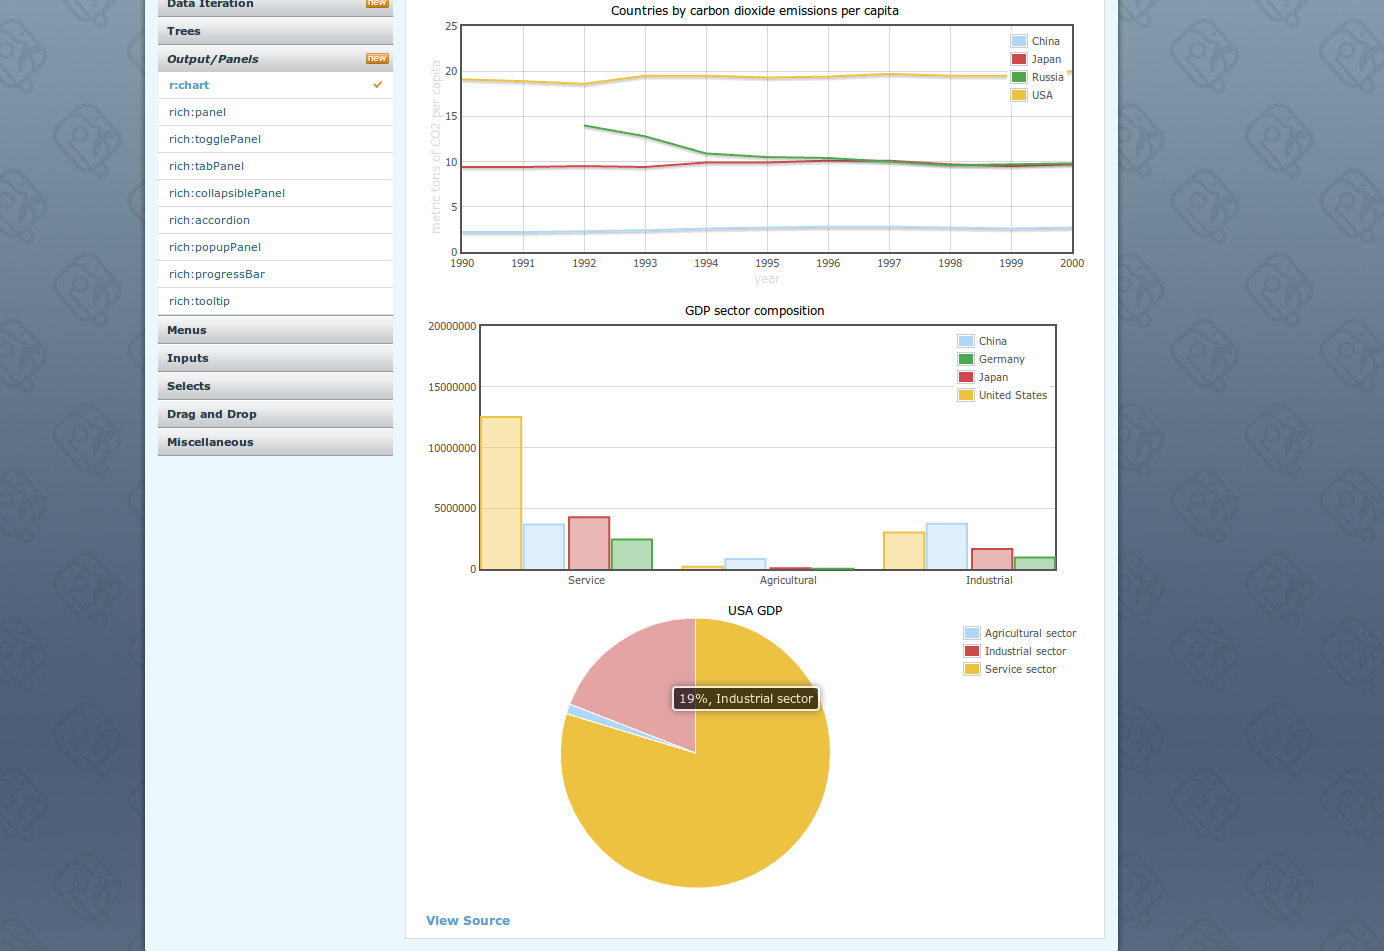
\includegraphics[width=0.9\textwidth]{figures/RichFacesShowcaseChartComponent.png}}}
    \end{center}
    \caption{RichFaces chart component shown in Showcase application}
    \label{fig:richfaces_chart} 
  \end{figure*}
  
  \section{Need for automation}
  The chapter \ref{sec:visual-testing-in-release-process} tried to outline how tedious and error prone might manual visual testing be. From our experience in the RichFaces QE team, any activity
  which needs to be repeated, and does not challenge tester's intellect enough, become a mundane activity. The more one repeats the mundane activity, the more likely an mistake is introduced:
  one forgets to try some use cases of an application, overlooks some minor errors, etc.
  
  Automated visual testing addresses this shortcomings, as it would unburden human resources from mundane activities such as manual testing, and would allow spending their
  time on intellectually more demanding problems. However, it introduces another kind of challenges, and needs to be implemented wisely. Following are minimal requirements 
  for a successful deployment of an automated visual testing.
      
  \section{Requirements for automation}
  \label{sec:requirementsForAutomation}
  An overall cost of the automation has to be taken into consideration. It is necessary to take into account higher initial cost of automation, and consequences it brings: 
  such as increased time to process relatively huge results of testing, cost of test suite maintenance.
  
  Therefore, to foster an effectiveness in quality assurance teams, while keeping the cost of automation reasonable low, automated visual testing would require:
  \begin{enumerate}
   \item A low cost of a test suite maintenance;
   \item a low percentage of false negative or false positive tests results;
   \item a reasonable time to execute the test suite;
   \item a concise yet useful test suite output;
   \item a support for Continuous Integration systems\footnote{Continuous Integration (CI) system is software to facilitate a practice of CI, which in short is about merging 
	  all developer copies with a shared mainline several times a day [5].}.
  \end{enumerate}
  
    \subsection{Low cost of test suite maintenance}
    A test suite needs to reflect a development of an application under test. Therefore, with each change in the application, it is usual that the test suite has to be changed as well.
    Making a change in the test suite can often introduce a bug, and cause false negative or false positive tests results.
    
    To keep this cost as low as possible, the test suite script has to be readable and meaningful, so when the change is about to be introduced, it is clear where and how it should be done.
    
    A test framework in which the test suite is developed should provide high enough abstraction. That would enable better re-usability for various parts of the test suite, 
    while lowering the overall cost of maintenance.
    
    Specifically for visual testing, when done by comparing screen captures, it is very important how well a repository of screen captures is maintainable. Secondly, 
    how reference (those correct ones, other screen captures will be compared with) screen captures are made.
    
    \subsection{Low percentage of false negative or false positive results}
    False negative test results incorrectly indicate a bug in an application under test, while it is a bug in the test suite itself. They are unwanted phenomenon as they take time to process
    and assess correctly.
    
    False positive tests results hide actual bugs in an application. They provide an incorrect feedback by showing the tests as passing, even when there is a bug in the application.
    
    Specifically for visual testing, when it is done by comparison of screen captures, it is very easily to be broken by small changes on a page. For example if the page outputs a current
    date, then it would break with every different date. There has to exist techniques, which would prevent these situations.
    
    \subsection{Reasonable time to execute a test suite}
    Reasonable time is quite subjective matter, but in general, it depends on how many times e.g. per day one needs to run whole test suite. Nowadays trend is a Continuous Integration,
    when a developer or a tester commits changes of an application several times per day to a shared source code mainline. Each such commit should trigger the test suite, which verifies 
    whether the change did not introduced an error to the application.
    
    According to creators of Continuous Integration practice, the whole point of CI is to provide a rapid feedback. A reasonable time for them is 10 minutes. If the build
    takes more time, every minute less is a huge improvement (considering a developer/tester runs test suite several times a day).
    
    \subsection{Concise yet useful test suite output}
    One of drawbacks of automated testing is its ability to produce huge amount of logs, test results etc. The output therefore needs to be as concise as possible, while still providing
    an useful information. A tester needs to be able to quickly recognize where the issue might be. The best situation would be if the tester does not need to run the test again in order
    to spot the issue. The output should give him a clear message where the issue is.
    
    For visual testing specifically, this can be achieved by providing a tester with screen captures together with difference of old and new version.
    
    \subsection{Support for Continuous Integration systems}
    This is quite easily to be achieved, but still, a developer of a tool for visual testing should have this in mind beforehand. Todays CI systems support variety of build systems, for
    various platforms, and languages. For example Jenkins supports build systems like Maven or Gradle, but it can run also shell scripts.
    
    
\chapter{Analysis of existing solutions}
As we introduced in \ref{sec:requirementsForAutomation}, there are many aspects which need to be taken into consideration when automating visual
testing. Following analysis is going to compare existing solutions to automated testing with those requirements in mind. We also focused on introducing
different approaches to visual testing.

The representative list of tools for comparison was made also according to an ability to be used in enterprise context. In enterprise there
is a stress on stability and reliability of employed solutions. It is quite vague requirement, and it is usually hard to find out which tools
are a good fit for an enterprise, however, some indicators, which we used as well, might be helpful:
\begin{itemize}
 \item Is a project actively developed? When was the last release of the project, or how old is the last commit to a source code mainline?
 \item How many opened issues the project has? When was the last activity with those issues ?
 \item What is the quality of the source code? Is it well structured? Does it employ best development practices?
 \item Does the project have a user forum? How active are the users?
 \item Is a big enterprise behind the solution, or otherwise sponsoring it ?
 \item What are the references if the project is commercialized ?
\end{itemize}

For each tool in following sections we are going to show an example usage and its main drawbacks together with some basic description.
  
  \section{Mogo}
  Mogo [6] approach to visual testing can be in short described like: 
  \begin{enumerate}
   \item One provides set of URLs of an application under test to a cloud based system.
   \item Application URLs are loaded in various browsers, detection of broken links is done.
   \item Screenshots are made and are compared with older screenshots from the same URL to avoid CSS regressions.
  \end{enumerate}
  
  There is no programming script required, therefore it can be used by less skilled human resources.
  
  Drawbacks of this approach are evident when testing dynamic pages, which content is changed easily. Applications which provide rich interaction options to an end user, and which state
  changes by interacting with various web components (calendar widget, table with sorting mechanism etc.), require more subtle way of configuring what actions need to be done before the
  testing itself. Mogo is suitable for testing static web applications, not modern AJAX enabled applications full of CSS transitions.
  
  Above mentioned drawbacks might lead to a bigger number of false negative test results when used with real data (any change, e.g. showing actual date may break testing), or to a bigger 
  number of false positive tests results when such a tool is used to test mocked data \footnote{Mocked data is made up data for purpose of testing, so it is consistent and does not change
  }.
  
  \section{BBC Wraith}
  Wraith is a screenshot comparison tool, created by developers at BBC News [7]. Their approach to visual testing can be described like:
  \begin{enumerate}
   \item Take screenshots of two versions of web application with use of either PhantomJS \ref{subsec:phantomCSS}, or with use of SlimerJS\footnote{SlimerJS is 
   very similar to PhantomJS \ref{subsec:phantomCSS}, it just runs on top of Gecko engine, which e.g. Mozilla Firefox runs on top of. [10]}.
   \item One version is the one currently developed (which run on localhost\footnote{In computer networking, localhost means this computer. [11]}), and the other one is a live site.
   \item Once screenshots of web page from these two different environments are captured a command line tool \texttt{imagemagic} is executed to compare screenshots.
   \item Any difference is marked with blue color in a created picture, which is the result of comparing two pictures (It can be seen at Figure \ref{fig:bbcWraithDiff}).
  \end{enumerate}
  
  \begin{figure*}[!htb]
    \begin{center}
    \leavevmode
    \centerline{\scalebox{1.0}{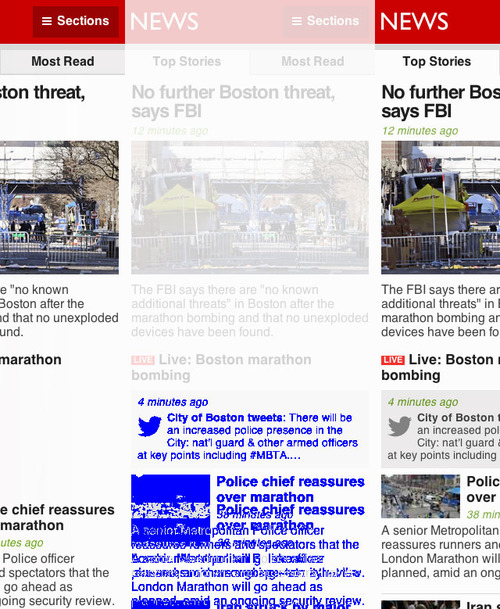
\includegraphics[width=0.4\textwidth]{figures/bbcWraith.jpg}}}
    \end{center}
    \caption{BBC Wraith picture showing difference in comparison of two web page versions}
    \label{fig:bbcWraithDiff} 
  \end{figure*}

  
    \subsection{PhantomCSS}
    \label{subsec:phantomCSS}
    PhantomCSS [8] is stack of web technologies based on headless\footnote{Headless software do not require graphical environment (such as X Windows system) for its execution.} 
    WebKit\footnote{WebKit is a layout engine software component for rendering web pages in web browsers, such as Apple's Safari or previously a Google Chrome [9]} engine, which can be 
    interacted with by using of its JavaScript API.
    
    For the sake of simplicity we can say that it is a browser which does not make any graphical output, which makes it a bit faster and less computer resource demanding tool.
    
    One can instruct PhantomCSS to take a screenshot of a web page with following script:
  
    \begin{verbatim}
      var page = require('webpage').create();
      page.open('http://google.com/', function() {
        page.render('google.png');
        phantom.exit();
      });
    \end{verbatim}
  
  \section{Facebook Huxley}
  
  \section{Rusheye}
  
  \section{Conclusion of analysis}
  Conclusion of drawbacks, and why we try to propose another approach
  
\chapter{New approach}
  
  \section{Hypothesis}
  Simply: reuse of functional tests of the application for visual testing
  
  \section{Process}
  How one would use my tool and where in testing stack such visual testing has its place, written in business process notation
  
  \section{Analysis of useful tool output}
  Requirements for useful output of such a tool based on questionnaire for RichFaces team, or maybe I will ask all JBoss employees
  
\chapter{Implemented tool}
An answer to the new process, requirements: CI viable, reusing what can be reused, extensible, cloud ready, multiple users

  \section{Client part}
  
    \subsection{Arquillian}
    Integration testing, starting containers, event based machine
  
    \subsection{Arquillian Graphene}
    Functional testing of Web UI, screenshooter
  
    \subsection{Rusheye}
    Screenshots comparison, rewritten to Arquillian core
  
    \subsection{Graphene visual testing}
    An adaptor between Rusheye and Arquillian Graphene
  
  \section{Server part}
  
    \subsection{Web application to view results}
    Its architecture, reasoning for chosen solutions, screenshots of app, key functionality
    
    \subsection{Storage of patterns}
    Description of solution, reasoning
    
\chapter{Deployment of tool and process}

  \section{Deployment on production application}
  Deployment on stable app
  
  \section{Deployment on development application}
  Deployment sooner on application which is in Alpha phase, my hypothesis is that it will not be worth to deploy it on such a app, due to too many changes
  
  \section{Usage with CI}
  Jenkins job and its cooperation with the tool, more particullary tool ability to handle multiple jobs, apps, versions, etc.
  
  \section{Cloud ready}
  The app can be easily deployed on Openshift
  
  \section{Results}
  The percentage of improvement of QA effectiveness
  
\chapter{Conclusion}
What I developed, What I improved, What can be better, Possible ways of extensions: Openshift cartridge
    
    % bibtex here
    \addcontentsline{toc}{chapter}{Bibliography}
    \pagestyle{plain}
    \bibliography{thesis}
    %[1] Hetzel, William C., The Complete Guide to Software Testing, 2nd ed. Publication info: Wellesley, Mass. : QED Information Sciences, 1988. ISBN: 0894352423.Physical description: ix, 280 p. : ill ; 24 cm.
    %[2] http://en.wikipedia.org/wiki/Waterfall_model
    %[3] http://en.wikipedia.org/wiki/Scrum_(software_development)
    %[4] http://www.w3schools.com/browsers/browsers_stats.asp
    %[5] http://en.wikipedia.org/wiki/Continuous_integration
    %[6] http://mogotest.com/
    %[7] https://github.com/BBC-News/wraith 
    %[8] http://phantomjs.org/
    %[9] http://en.wikipedia.org/wiki/WebKit
    %[10] http://slimerjs.org/
    %[11] http://en.wikipedia.org/wiki/Localhost
    %[12] http://media.tumblr.com/c5bf7caefde043ee7532b641c7f0e157/tumblr_inline_moaf774b5i1qz4rgp.jpg

\end{document}